\section{Instalación y configuración de Kubuntu}
\label{instKubuntu}

En esta sección se describe el proceso de instalación y configuración de Kubuntu 8.04 (Hardy Heron).

\subsection{Instalación de Kubuntu}

En primer lugar hay que configurar el ordenador para que arranque desde la unidad de CD. A continuación se introduce el disco de Kubuntu en el lector y se reinicia el equipo para empezar el proceso de instalación.

Los pasos a realizar para llevar a cabo la instalación son los siguientes:

\begin{enumerate}
 \item Selección de idioma para el proceso de instalación (español, en este caso)
\begin{figure}[htb!]
 \centering
 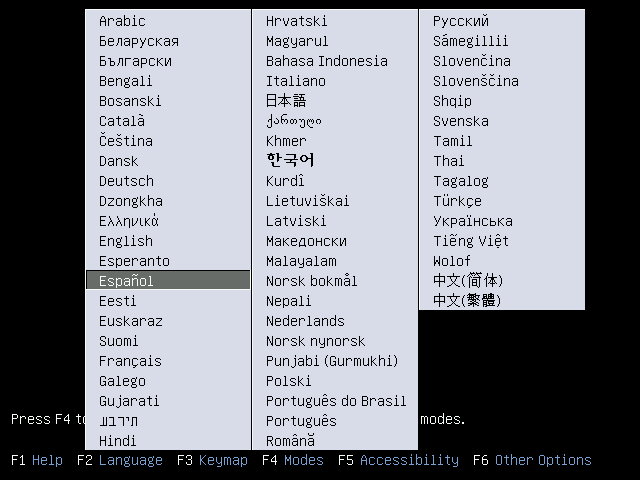
\includegraphics[width=0.8\textwidth]{Utils/instalacion1.png}
 % instalacion1.png: 1179668x1179666 pixel, 0dpi, infxinf cm, bb=
 \caption{Selección de idioma de la instalación}
 \label{fig:instalacion1}
\end{figure}

\item Seleccionar la opción ``Instalación de Kubuntu'' en el menú

\item Elección de ubicación (España en el caso que nos ocupa)

\begin{figure}[htb!]
 \centering
 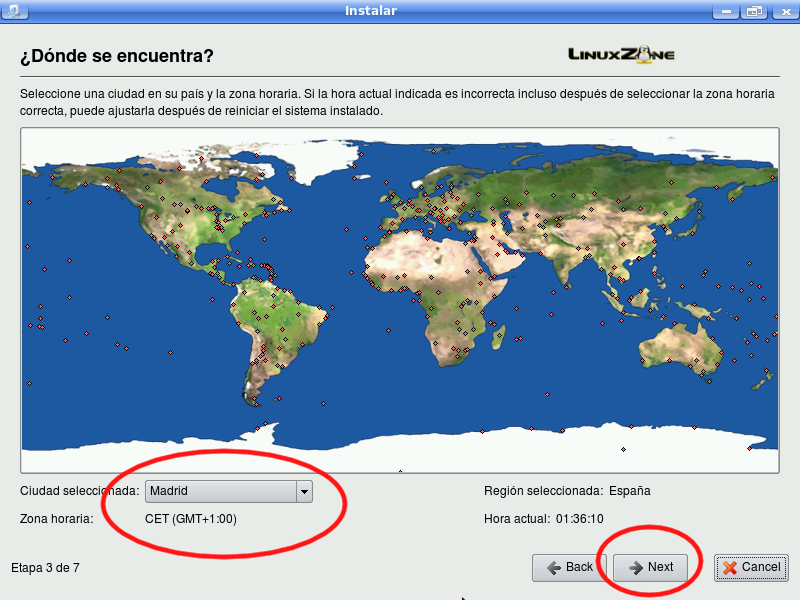
\includegraphics[width=0.8\textwidth]{Utils/instalacion4.png}
 % instalacion1.png: 1179668x1179666 pixel, 0dpi, infxinf cm, bb=
 \caption{Selección de la ubicación}
 \label{fig:instalacion4}
\end{figure}

\item Selección del modelo de teclado (español).

\item Detección de hardware, descarga de componentes adicionales necesarios y configuración de red (procesos automáticos).

\item Particionado del sistema. Es posible mantener particiones que contengan otros sistemas operativos, aunque en este caso se destinará toda la capacidad del disco a Kubuntu. Para ello se elegirá el particionado manual y se eliminarán todas las particiones existentes. A continuación se crearán tres particiones utilizando el gestor de particiones mostrado en la Figura \ref{fig:particionado}:
\begin{itemize}
 \item Partición de 19GB con sistema de ficheros ext3 y punto de montaje en ``/''.
 \item Partición de 60Gb con sistema de ficheros ext3 y punto de montaje en ``/home''.
 \item Partición de  1GB de tipo swap (intercambio).
\end{itemize}

\begin{figure}[htb!]
 \centering
 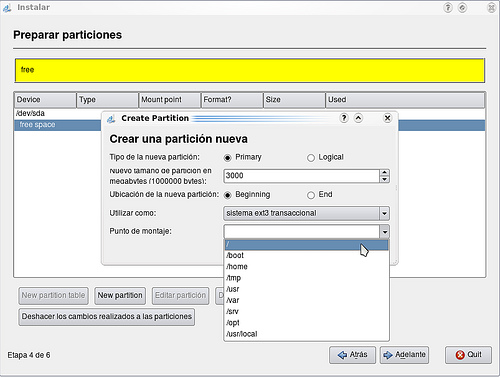
\includegraphics[width=0.8\textwidth]{Utils/particionado.png}
 % instalacion1.png: 1179668x1179666 pixel, 0dpi, infxinf cm, bb=
 \caption{Particionado del sistema}
 \label{fig:particionado}
\end{figure}

\item Creación del sistema de archivos ext3 e instalación del sistema base Kubuntu. Descarga del resto de paquetes necesarios a disco, incluyendo el soporte para el idioma español. (Proceso automático.)

\item Introducción del nombre del administrador del sistema, nombre de usuario y contraseña y nombre del equipo.

\item Fin de la instalación inicial de Kubuntu. Es necesario extraer el disco del lector de CD y reiniciar el sistema. Este primer arranque será bastante más lento de lo habitual ya que se descargarán e instalarán numerosos paquetes.
\end{enumerate}

\newpage
Una vez hecho introducidos todos los datos y guardados los cambios la conexión a
Internet ya estará activa.